\documentclass[11pt,a4paper]{article}
\usepackage[margin=2.4cm]{geometry}
\usepackage{fontspec}
\usepackage{booktabs}
\usepackage{amsmath}
\usepackage{xcolor}
\usepackage{tikz}
\usetikzlibrary{positioning,arrows.meta,shapes.misc,calc}
\usepackage{enumitem}
\usepackage{hyperref}
\usepackage{microtype}
\usepackage{needspace}
\usepackage{graphicx}
\usepackage{amssymb}
\usepackage{longtable}
\usepackage{array}
\setlength{\parskip}{6pt}
\setlength{\parindent}{0pt}
\definecolor{pink}{HTML}{CF1A5C}
\definecolor{blue}{HTML}{2D6BB5}
\definecolor{grey}{HTML}{7D8893}
\definecolor{ink}{HTML}{101820}
\hypersetup{colorlinks=true,linkcolor=blue,urlcolor=blue}

\title{\Huge Teaching a Computer to Point at the Right Part of a Drawing\\[6pt]
\Large Every experiment so far, what we kept, what we threw away, and how the latest one does, in simple words}
\author{SVG Patch Lab}
\date{10 September 2026}

\begin{document}
\maketitle

\section*{The problem, in one picture}

An SVG is a drawing made of lines. Each line has a name: \texttt{n1}, \texttt{n2}, \texttt{n3}, and so on.
Someone types an instruction like \emph{``Change the camera lens to red.''}
The computer has to answer one question: \textbf{which line is the lens?}

\begin{center}
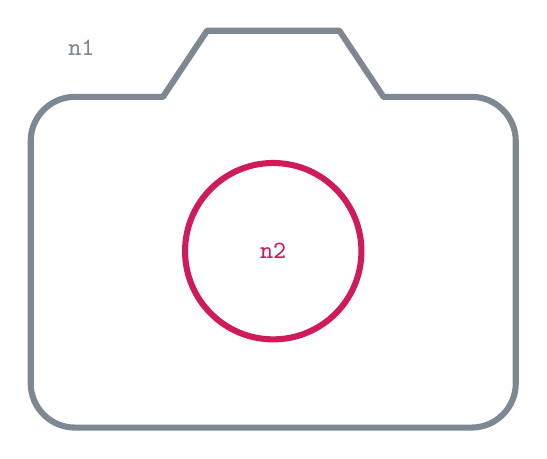
\begin{tikzpicture}[line width=2.2pt, line cap=round, line join=round, scale=0.28]
  % camera body (n1), drawn in grey
  \draw[grey] (23,5) .. controls (23,3.9) and (22.1,3) .. (21,3) -- (3,3) .. controls (1.9,3) and (1,3.9) .. (1,5) -- (1,16) .. controls (1,17.1) and (1.9,18) .. (3,18) -- (7,18) -- (9,21) -- (15,21) -- (17,18) -- (21,18) .. controls (22.1,18) and (23,17.1) .. (23,16) -- cycle;
  % lens (n2), in pink
  \draw[pink] (12,11) circle (4);
  \node[grey, font=\ttfamily\small] at (3.3,20.2) {n1};
  \node[pink, font=\ttfamily\small] at (12,11) {n2};
\end{tikzpicture}

\small The camera icon from the Feather set. The body is \texttt{n1}; the lens is \texttt{n2}.
\end{center}

If the computer points at the right line, we can change its colour safely and nothing else in the drawing is touched.
If it points at the wrong line, the drawing breaks.
So the whole game is \textbf{pointing at the right line}.

\section*{Why we did this experiment}

Before today, our pointing brain got the right answer on only \textbf{22 out of 100} new drawings.
When we looked at the mistakes, \textbf{48 of them were ``wrong part''} mistakes: it pointed at the camera body when asked for the lens, or at the battery when asked for the lightning bolt.

Why? The old brain was trained only on \emph{made-up practice drawings} where the instructions used simple words like ``the red circle on the left''.
It had never seen the words \emph{lens}, \emph{lightning bolt}, \emph{bell}, or \emph{hull}.
When it heard a word it did not know, it just guessed the biggest line.

So the idea was simple: \textbf{add a helper that already knows what things look like.}

\section*{The data we used}

There are three piles of drawings. Keeping them apart is the most important rule.

\begin{description}[leftmargin=1.6em, style=nextline]
  \item[1. Practice drawings (made up by a program).] Thousands of simple scenes with instructions like ``the small blue square''. The old brain learned from these. Nothing new was trained today, so today they were only used to make the old brain's scores.
  \item[2. The old test (80 drawings).] Real icons from two collections called Hicon and Streetmix, with real instructions from a public dataset (VectorEdits). Their right answers were worked out automatically by comparing the before and after drawings, so they are a bit rough. We used this pile like a \emph{practice exam}: to choose one knob (see below) and nothing else.
  \item[3. The real test (100 instructions on 50 icons).] Icons from two collections called Feather and Tabler that nobody in this project had used before. Two instructions were written for each icon, for example ``Change the clock hands to red''. Every right answer was checked by eye in the drawing. 45 of the 100 answers need \emph{more than one line} (for example both wheels of a truck). This pile is \textbf{sealed}: a fingerprint (a hash) of the file is stored, and the program refuses to run if the file changes. Nobody tunes anything on it. Today was the third time it was ever scored.
\end{description}

\section*{The pictures in the data}

\subsection*{The sealed test}
Thirty of the 100 instructions. Pink is the right answer; the small text says which lines and how many there were to choose from.

\begin{center}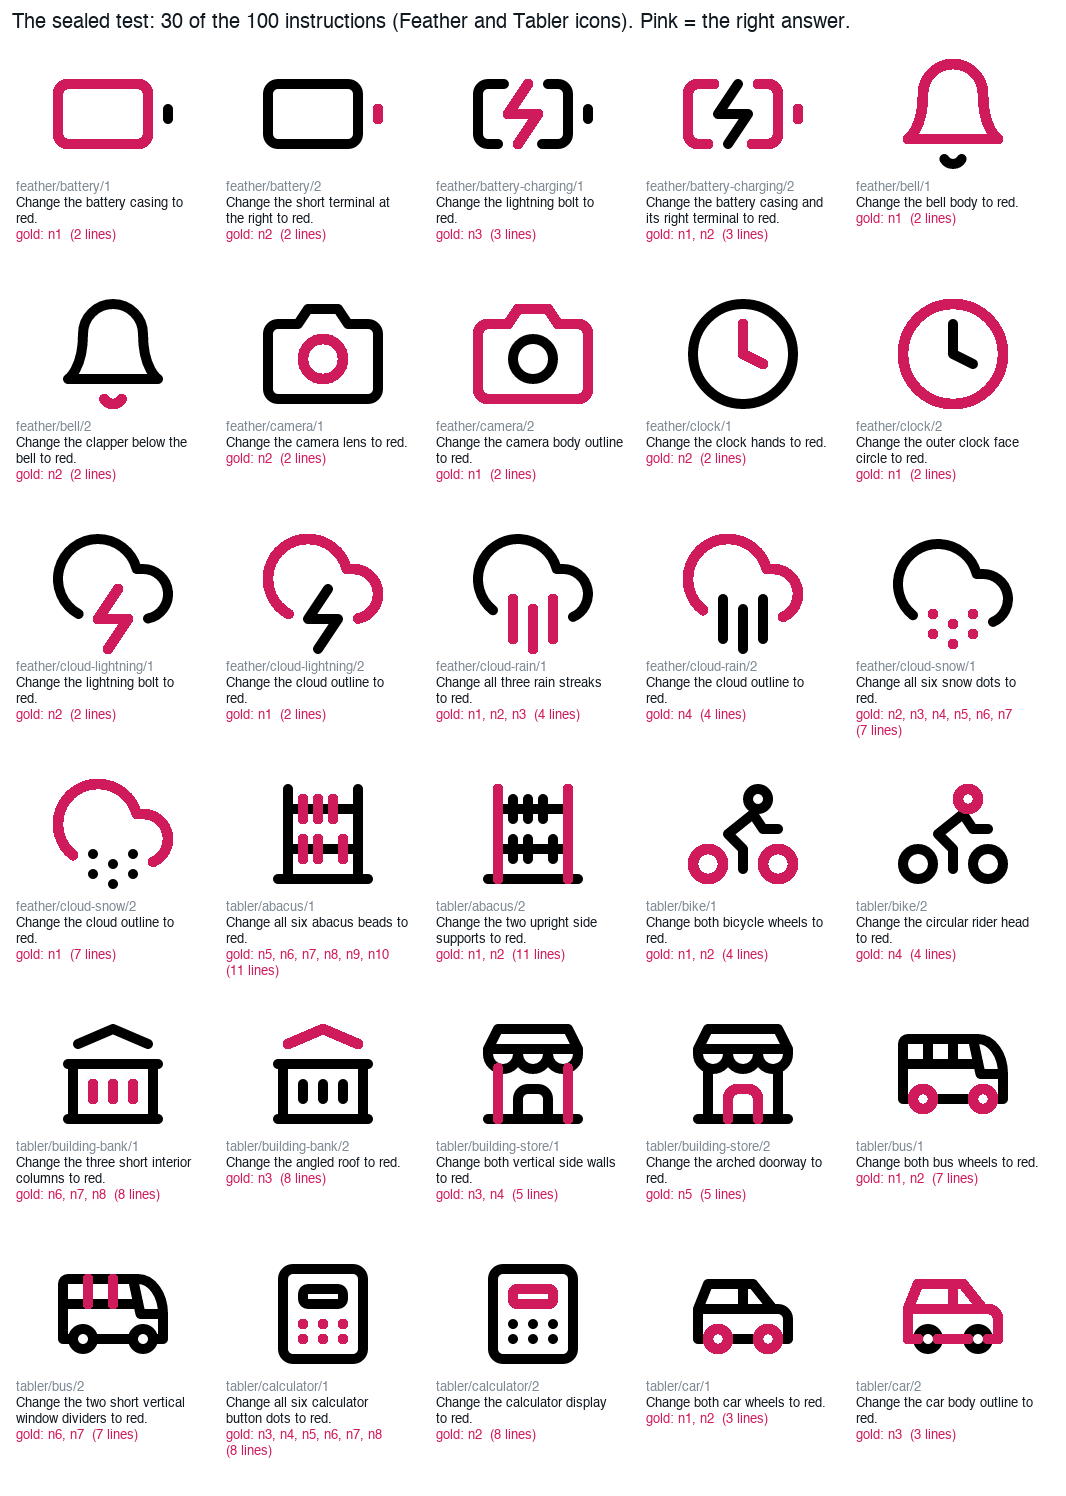
\includegraphics[width=\textwidth]{img/dataset_holdout.png}\end{center}

\subsection*{What the helper saw}
For every line, three little pictures and the words for the part. This is the whole input to SigLIP.

\begin{center}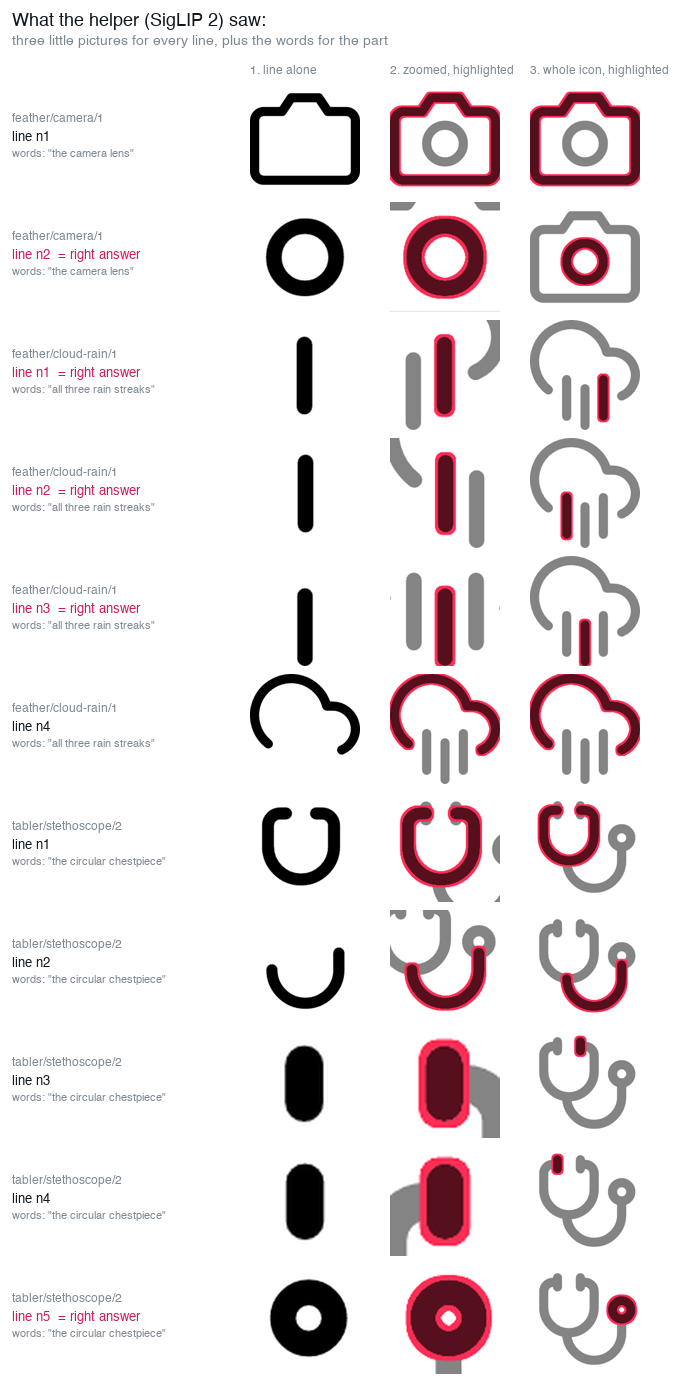
\includegraphics[height=0.86\textheight]{img/dataset_siglip_views.png}\end{center}

\subsection*{The practice exam}
Twelve of the 80 VectorEdits icons. They look different from the test (dense filled icons and street scenes), which is one reason a sealed test was needed.

\begin{center}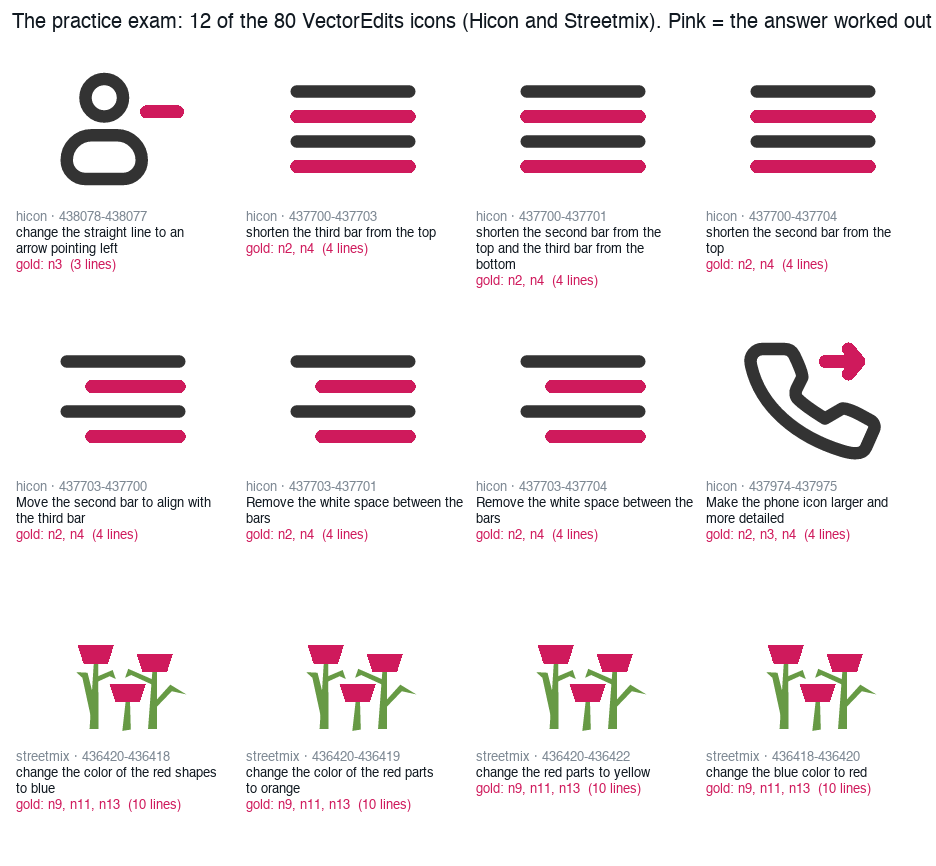
\includegraphics[width=\textwidth]{img/dataset_practice80.png}\end{center}

\subsection*{The made-up training drawings}
Twelve of the 2{,}380 program-made scenes the old brain learned from. The words are colours, positions and simple parts. ``Lens'' and ``clapper'' never appear.

\begin{center}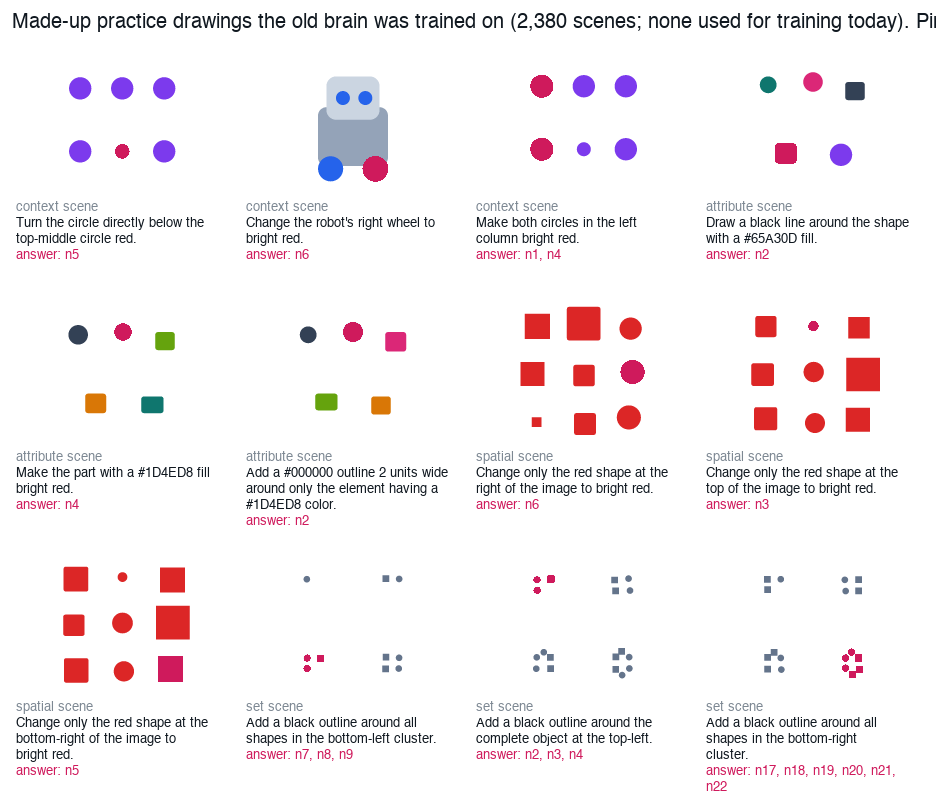
\includegraphics[width=\textwidth]{img/dataset_synthetic.png}\end{center}

\section*{The pieces of the machine}

\subsection*{The old brain (a small neural network)}

The old brain is a tiny network (a ``no-edge MLP''). For each line in the drawing it looks at numbers: how big the line is, where it sits, what colour it has, what kind of shape it is.
It reads the instruction with a cheap trick called \emph{hashing}, which turns words into numbers without understanding them.
It gives every line a score from 0 to 1, and it has a second little part, the \textbf{count head}, that guesses \emph{how many} lines to pick.
Then it sorts the lines by score and picks the top ones.
It is frozen: we did not change it at all today.

\subsection*{The new helper (SigLIP 2)}

SigLIP 2 is a big model that Google trained on hundreds of millions of pictures with captions.
It can look at a picture and a sentence and say \emph{how well they match}.
We did not train it either. We just use it.

For each line in a drawing we make three small pictures:
\begin{itemize}[leftmargin=1.6em]
  \item the line \textbf{alone} on a white background,
  \item a \textbf{zoomed-in} view with that line highlighted in pink,
  \item the \textbf{whole icon} with that line highlighted in pink.
\end{itemize}
We show all three pictures and the words that name the part (``the camera lens'') to SigLIP.
It gives a matching score for each line. The three pictures are mixed with fixed weights (half, a third, and a fifth) that were chosen in an earlier experiment and left alone.

\subsection*{Mixing the two, with one knob}

Now every line has two scores: one from the old brain and one from the helper.
We add them together with one knob called $\alpha$ (alpha) between 0 and 1:

\[
\text{final score} \;=\; (1-\alpha)\times(\text{old brain's score}) \;+\; \alpha\times(\text{helper's score}).
\]

$\alpha = 0$ means ``only the old brain''. $\alpha = 1$ means ``only the helper''.
(The two scores live on different scales, so under the hood the old brain's score is turned into a \emph{logit} and the helper's is multiplied by SigLIP's own built-in scale of about 113. That is just so they can be added fairly.)

\textbf{How we chose the knob.} We tried eleven values of $\alpha$ on the \emph{practice exam} (the 80 old drawings) and wrote down, \emph{before} looking, the rule for picking the winner: the value that gets the most drawings exactly right.
$\alpha = 0$ gave 41 out of 80, exactly what the old brain got before, which proved the pipeline was wired correctly.
The winner was $\alpha = 0.7$. We saved it in a config file, committed it to git, and only then ran the real test.
The program refuses to score the real test unless the knob is already frozen in that file.

\subsection*{The last step is unchanged}

After mixing, we sort the lines by final score and take the top $k$, where $k$ comes from the old count head.
Same as before. This matters: today's experiment only changed \emph{which lines come first}, not \emph{how many} are taken.

\begin{center}
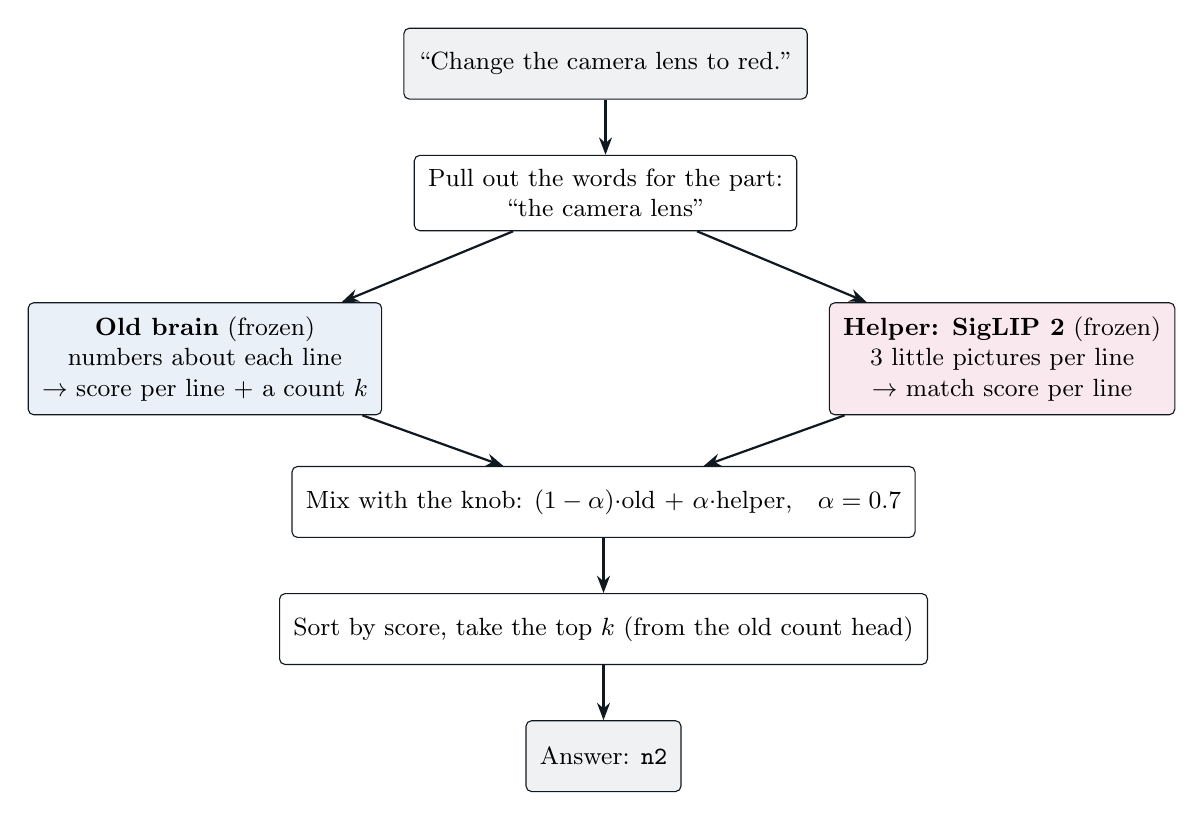
\begin{tikzpicture}[
  node distance=7mm and 9mm,
  box/.style={draw=ink, rounded corners=2pt, align=center, font=\small, inner sep=5pt, minimum height=9mm},
  arrow/.style={-{Stealth[length=2.2mm]}, line width=0.8pt, ink}
]
  \node[box, fill=grey!12] (instr) {``Change the camera lens to red.''};
  \node[box, below=of instr] (phrase) {Pull out the words for the part:\\``the camera lens''};
  \node[box, below left=9mm and 4mm of phrase, fill=blue!10] (mlp) {\textbf{Old brain} (frozen)\\numbers about each line\\$\to$ score per line + a count $k$};
  \node[box, below right=9mm and 4mm of phrase, fill=pink!10] (sig) {\textbf{Helper: SigLIP 2} (frozen)\\3 little pictures per line\\$\to$ match score per line};
  \node[box] (mix) at ($(mlp.south)!0.5!(sig.south) + (0,-11mm)$) {Mix with the knob: $(1-\alpha)\cdot$old $+\ \alpha\cdot$helper,\quad $\alpha = 0.7$};
  \node[box, below=of mix] (pick) {Sort by score, take the top $k$ (from the old count head)};
  \node[box, below=of pick, fill=grey!12] (ans) {Answer: \texttt{n2}};
  \draw[arrow] (instr) -- (phrase);
  \draw[arrow] (phrase) -- (mlp);
  \draw[arrow] (phrase) -- (sig);
  \draw[arrow] (mlp) -- (mix);
  \draw[arrow] (sig) -- (mix);
  \draw[arrow] (mix) -- (pick);
  \draw[arrow] (pick) -- (ans);
\end{tikzpicture}
\end{center}

\needspace{14\baselineskip}
\section*{What happened}

We ran the real test once. Here is what each version of the machine got exactly right.

\begin{center}
\small
\begin{tabular}{@{}lrrrr@{}}
\toprule
Version & Right / 100 & One-line / 55 & Many-line / 45 & Wrong part \\
\midrule
Old brain (the baseline) & 22 & 18 & 4 & 48 \\
Trained top-$k$ head (yesterday's best) & 27 & 23 & 4 & 50 \\
Trained head + group choices & 23 & 19 & 4 & 52 \\
Helper only ($\alpha = 1$) & 37 & 36 & 1 & 26 \\
\textbf{Old brain + helper ($\alpha = 0.7$)} & \textbf{39} & 35 & 4 & 28 \\
\bottomrule
\end{tabular}
\end{center}

In plain words:
\begin{itemize}[leftmargin=1.6em]
  \item The mix went from 22 to \textbf{39} right answers. That is 17 more. Even after allowing for luck (a statistical check that shuffles the icons 5{,}000 times), the gain is somewhere between 10 and 24. It is real.
  \item It beat yesterday's best system, which had actually been \emph{trained}, by 12. Today's addition was not trained at all.
  \item Wrong-part mistakes fell from 48 to 28.
  \item It fixed 19 drawings and broke 2. The 19 were all about words: bolt, bell, hull, antenna, chestpiece. The 2 it broke were tiny marks described by position (``the small dot below the arcs''), where the old brain had been right.
  \item Helper-only got 37, almost as good, but it loses the many-line answers (1 instead of 4). Mixing keeps them.
\end{itemize}

\section*{Everything we tried before, and what happened to it}

The latest experiment stands on a pile of older ones. Here is the whole pile, oldest first, with the number each one produced and what we did with it.
``Kept'' means the idea is still inside today's machine. ``Dropped'' means we stopped using it, and the reason is written next to it.

\subsection*{1. Giving a language model numbers about each line (July--August)}

At first the pointing was done by a large language model (Qwen, 7 billion parameters) that read a text summary of the drawing.
We tried adding, for every line, about twenty numbers that come from actually drawing the picture: where the line paints, how big it is, its colour.
To get those numbers we draw the picture once with the line and once without it and look at the difference.

\begin{itemize}[leftmargin=1.6em]
  \item \textbf{Two small A/B tests.} With the numbers, the model won 6--0 and then 10--0 on the drawings where the two versions disagreed. \textbf{Kept:} the ``what do you look like and where are you'' numbers still feed the old brain today.
  \item \textbf{The hide-and-seek test} (48 drawings where one shape covers another). Plain geometry got 0 of 24 hidden cases; the drawn numbers got 9 of 24. \textbf{Kept:} drawing the picture is worth it exactly when the raw numbers lie.
  \item \textbf{Can every line even be seen?} We checked 300 emoji and 300 real clip-art files. 98.9\% of emoji lines have their own pixels; only 58.7\% of clip-art lines do. Two in five clip-art lines cannot be told apart by \emph{any} picture method. \textbf{Kept as a warning:} a pointer that always answers is pretending.
  \item \textbf{Why we moved on:} sending those numbers for every line made the prompts long and made colour edits \emph{worse}, and a 7-billion-parameter model is expensive. The next question was whether a tiny brain with no language model could point at all.
\end{itemize}

\subsection*{2. The Graph-MoE brain on made-up drawings (early September)}

We built a tiny brain that reads the instruction with the hashing trick, sends it to a ``colour expert'' or a ``position expert'', and scores each line.
One version passes messages between neighbouring lines in the drawing (a graph network, ``GNN''); the other does not (the ``no-edge MLP'').

\begin{itemize}[leftmargin=1.6em]
  \item On 59 made-up test drawings the GNN got 58 right and the MLP got 51. The GNN won 8--1 on ``the one to the left of'' type questions. It looked like the graph helped.
  \item Glued to simple rules, the brain got 500 of 500 edits exactly right on five tasks of the public SVGEditBench benchmark, with no language model at all. \textbf{But} this is because those instructions name the colour that is already in the file; it proves the plumbing works, not that the brain understands pictures.
\end{itemize}

\subsection*{3. First real drawings: 80 icons from VectorEdits}

\begin{itemize}[leftmargin=1.6em]
  \item \textbf{Read the whole sentence, or just the part?} ``Rotate the arrow to point left'' -- the word \emph{left} is where the arrow should go, not where it is. Pulling out just ``the arrow'' before pointing took the MLP from 12 to 30 right answers (when told how many lines to pick). \textbf{Kept:} we always pull out the part's words first.
  \item \textbf{GNN on real icons:} 19 of 80 versus the MLP's 30. The graph was already falling behind on real drawings.
  \item \textbf{Picking lines by a score cut-off:} at best 4 of 80. \textbf{Dropped:} a cut-off cannot tell how many lines a part has. This is why the count head was built.
  \item \textbf{The helper (SigLIP) on its own:} 41 of 80 top picks right. Poor on the dense Hicon icons (14 of 64), very good on Streetmix scenes (14 of 16). The old brain and the helper were right on \emph{different} drawings: together they could cover 55 of 80. \textbf{Kept for later:} this is the seed of today's experiment.
  \item \textbf{A switch: use the helper only for busy drawings} (ten or more lines). 66 of 80 top picks. \textbf{Dropped:} the switch line fell exactly between the two collections, so it was really learning ``which collection is this'', not ``how busy is this''.
\end{itemize}

\subsection*{4. The matched GPU run: GNN versus MLP, with counting (9 September)}

Both brains were trained the same way, with a count head, and tested on the same 80 icons, plus a set of hand-written grouping rules (``if the instruction names a colour, take every line with that colour'' and similar) that step in when they are sure and stay quiet otherwise.

\begin{itemize}[leftmargin=1.6em]
  \item GNN + rules: 32 of 80. MLP + rules: \textbf{42 of 80}. Without rules: 17 versus 27. Over 15 re-runs with different random seeds the MLP won 14 times. \textbf{Dropped: the GNN.} Its advantage on made-up drawings did not carry over, and we never found out why.
  \item The grouping rules added 7 drawings (35 to 42). \textbf{Kept, but with a warning:} the rules were written while looking at these same 80 drawings. On the 100 new icons later, they never once spoke up.
  \item The Colab machine was switched off before the trained brains were downloaded. The numbers survived in the saved notebook; the weights did not. Lesson learnt: download first.
  \item \textbf{Decision:} freeze ``MLP + rules'' as the baseline and stop tuning on the 80. Build a new, sealed test.
\end{itemize}

\subsection*{5. The sealed test and the ``more choices'' idea (10 September, morning)}

The 100-instruction Feather/Tabler test was built and sealed.
Then an experiment: instead of picking lines one by one, let a small trained head pick from a list of \emph{ready-made sets} of lines. One version only saw simple sets (the top-1, top-2, \dots\ by score); the other also saw sets that the drawing's own structure suggests (lines inside the same group, lines with the same colour).

\begin{itemize}[leftmargin=1.6em]
  \item First run: simple sets 25, structure sets 25, old brain 22. Then an audit found a bug: during training the lists had contained invisible ``group'' wrappers that the test never offers. Fixed and re-run.
  \item Corrected run: simple sets \textbf{27}, structure sets \textbf{23}, old brain \textbf{22}. The structure sets contained the right answer more often (80\% versus 72\%) and still scored lower. \textbf{Dropped: structure sets.} Offering more choices does not help a chooser that cannot tell them apart.
  \item The corrected numbers were checked line by line today, and the run's console was recovered from Google Drive so the result has a paper trail.
  \item \textbf{What we learnt:} 48 of the 100 mistakes were ``wrong part''. The words were the problem, not the sets. That is what today's helper is for.
\end{itemize}

\subsection*{6. Today: the helper, and what we did not do}

\begin{itemize}[leftmargin=1.6em]
  \item Helper alone: 37 of 100. Old brain + helper: \textbf{39}. \textbf{Kept: the mix}, because the helper alone loses the many-line answers (1 of 45 against 4 of 45).
  \item Counting fixes tried on the practice exam only: at best 3 more of 80. \textbf{Not applied to the real test.}
\end{itemize}

\subsection*{All the numbers in one table}

\begin{center}
\footnotesize
\begin{tabular}{@{}p{1.5cm}p{4.9cm}p{2.5cm}rp{3.3cm}@{}}
\toprule
When & What & Test & Right & What we did \\
\midrule
Jul--Aug & Drawn numbers for a 7B language model & two A/Bs & 6--0, 10--0 & kept the numbers \\
Aug & Drawn numbers vs plain geometry & 24 hidden cases & 0 vs 9 & kept \\
Aug & Lines you can see at all & 300 + 300 files & 98.9\% vs 58.7\% & kept as a warning \\
Sep 6--8 & GNN vs MLP, made-up drawings & 59 & 58 vs 51 & GNN looked good \\
Sep 8 & Rules + brain on SVGEditBench & 500 & 500 & plumbing only \\
Sep 9 & Part words vs whole sentence (MLP) & 80, told $k$ & 12 $\to$ 30 & kept \\
Sep 9 & GNN, part words & 80, told $k$ & 19 & falling behind \\
Sep 9 & Score cut-off & 80 & 4 & dropped \\
Sep 9 & Helper alone & 80, top pick & 41 & kept for later \\
Sep 9 & Helper-only-when-busy switch & 80, top pick & 66 & dropped, post-hoc \\
Sep 9 & GNN + rules vs MLP + rules & 80 & 32 vs 42 & GNN dropped \\
Sep 9 & 15 seeds & 80 & MLP 14/15 & baseline frozen \\
Sep 10 & Set-picking heads, run 1 & 100 sealed & 25 / 25 / 22 & bug found \\
Sep 10 & Set-picking heads, corrected & 100 sealed & 27 / 23 / 22 & structure sets dropped \\
Sep 10 & Helper alone & 100 sealed & 37 & \\
Sep 10 & \textbf{Old brain + helper} & 100 sealed & \textbf{39} & \textbf{current best} \\
Sep 10 & Counting fixes & 80 practice & +3 & not applied \\
\bottomrule
\end{tabular}
\end{center}

\section*{Looking at real examples}

Eleven icons from the sealed test. In each row the left picture shows the right answer in pink. The middle picture shows what the old brain picked, the right picture what the mix picked, both in blue. Grey lines were not picked.

\subsection*{Fixed by the helper}
These needed a word the old brain had never seen. The helper knows what a bolt, a hull, a chestpiece and a headband look like.

\needspace{9\baselineskip}
\noindent\texttt{feather/battery-charging/1} \quad \emph{``Change the lightning bolt to red.''} \quad {\small\color{grey} 3 lines to choose from}\\[3pt]
\begin{center}
\begin{tabular}{@{}c@{\hspace{9mm}}c@{\hspace{9mm}}c@{}}

\includegraphics[width=2.6cm]{img/feather_battery-charging_1_gold.png} &

\includegraphics[width=2.6cm]{img/feather_battery-charging_1_base.png} &

\includegraphics[width=2.6cm]{img/feather_battery-charging_1_fused.png} \\
{\small Gold: \texttt{n3}} &
{\small Old brain: \texttt{n2} \textcolor{pink}{$\times$}} &
{\small Mix: \texttt{n3} \textcolor{blue}{\checkmark}} \\
\end{tabular}\\[-2pt]
{\small\color{grey} Mix's order: \texttt{n3 > n2 > n1} \quad count head said $k=1$}
\end{center}

\needspace{9\baselineskip}
\noindent\texttt{tabler/sailboat/1} \quad \emph{``Change the wavy water line to red.''} \quad {\small\color{grey} 4 lines to choose from}\\[3pt]
\begin{center}
\begin{tabular}{@{}c@{\hspace{9mm}}c@{\hspace{9mm}}c@{}}

\includegraphics[width=2.6cm]{img/tabler_sailboat_1_gold.png} &

\includegraphics[width=2.6cm]{img/tabler_sailboat_1_base.png} &

\includegraphics[width=2.6cm]{img/tabler_sailboat_1_fused.png} \\
{\small Gold: \texttt{n1}} &
{\small Old brain: \texttt{n3} \textcolor{pink}{$\times$}} &
{\small Mix: \texttt{n1} \textcolor{blue}{\checkmark}} \\
\end{tabular}\\[-2pt]
{\small\color{grey} Mix's order: \texttt{n1 > n2 > n4 > n3} \quad count head said $k=1$}
\end{center}

\needspace{9\baselineskip}
\noindent\texttt{tabler/stethoscope/2} \quad \emph{``Change the circular chestpiece to red.''} \quad {\small\color{grey} 5 lines to choose from}\\[3pt]
\begin{center}
\begin{tabular}{@{}c@{\hspace{9mm}}c@{\hspace{9mm}}c@{}}

\includegraphics[width=2.6cm]{img/tabler_stethoscope_2_gold.png} &

\includegraphics[width=2.6cm]{img/tabler_stethoscope_2_base.png} &

\includegraphics[width=2.6cm]{img/tabler_stethoscope_2_fused.png} \\
{\small Gold: \texttt{n5}} &
{\small Old brain: \texttt{n3} \textcolor{pink}{$\times$}} &
{\small Mix: \texttt{n5} \textcolor{blue}{\checkmark}} \\
\end{tabular}\\[-2pt]
{\small\color{grey} Mix's order: \texttt{n5 > n1 > n2 > n3 > n4} \quad count head said $k=1$}
\end{center}

\needspace{9\baselineskip}
\noindent\texttt{feather/headphones/2} \quad \emph{``Change the curved headband to red.''} \quad {\small\color{grey} 2 lines to choose from}\\[3pt]
\begin{center}
\begin{tabular}{@{}c@{\hspace{9mm}}c@{\hspace{9mm}}c@{}}

\includegraphics[width=2.6cm]{img/feather_headphones_2_gold.png} &

\includegraphics[width=2.6cm]{img/feather_headphones_2_base.png} &

\includegraphics[width=2.6cm]{img/feather_headphones_2_fused.png} \\
{\small Gold: \texttt{n1}} &
{\small Old brain: \texttt{n2} \textcolor{pink}{$\times$}} &
{\small Mix: \texttt{n1} \textcolor{blue}{\checkmark}} \\
\end{tabular}\\[-2pt]
{\small\color{grey} Mix's order: \texttt{n1 > n2} \quad count head said $k=1$}
\end{center}

\subsection*{Broken by the helper}
The old brain had these right. Both describe a tiny mark by where it is, and the three little pictures do not separate it from the arcs around it.

\needspace{9\baselineskip}
\noindent\texttt{feather/watch/1} \quad \emph{``Change the watch hands to red.''} \quad {\small\color{grey} 3 lines to choose from}\\[3pt]
\begin{center}
\begin{tabular}{@{}c@{\hspace{9mm}}c@{\hspace{9mm}}c@{}}

\includegraphics[width=2.6cm]{img/feather_watch_1_gold.png} &

\includegraphics[width=2.6cm]{img/feather_watch_1_base.png} &

\includegraphics[width=2.6cm]{img/feather_watch_1_fused.png} \\
{\small Gold: \texttt{n2}} &
{\small Old brain: \texttt{n2} \textcolor{blue}{\checkmark}} &
{\small Mix: \texttt{n3} \textcolor{pink}{$\times$}} \\
\end{tabular}\\[-2pt]
{\small\color{grey} Mix's order: \texttt{n3 > n2 > n1} \quad count head said $k=1$}
\end{center}

\needspace{9\baselineskip}
\noindent\texttt{feather/wifi/2} \quad \emph{``Change the small dot below the arcs to red.''} \quad {\small\color{grey} 4 lines to choose from}\\[3pt]
\begin{center}
\begin{tabular}{@{}c@{\hspace{9mm}}c@{\hspace{9mm}}c@{}}

\includegraphics[width=2.6cm]{img/feather_wifi_2_gold.png} &

\includegraphics[width=2.6cm]{img/feather_wifi_2_base.png} &

\includegraphics[width=2.6cm]{img/feather_wifi_2_fused.png} \\
{\small Gold: \texttt{n4}} &
{\small Old brain: \texttt{n4} \textcolor{blue}{\checkmark}} &
{\small Mix: \texttt{n2} \textcolor{pink}{$\times$}} \\
\end{tabular}\\[-2pt]
{\small\color{grey} Mix's order: \texttt{n2 > n4 > n3 > n1} \quad count head said $k=1$}
\end{center}

\subsection*{Right order, wrong count}
The mix puts every gold line first. Then the old count head takes too few (one) or too many (four).

\needspace{9\baselineskip}
\noindent\texttt{feather/save/1} \quad \emph{``Change the two interior panels of the floppy disk to red.''} \quad {\small\color{grey} 3 lines to choose from}\\[3pt]
\begin{center}
\begin{tabular}{@{}c@{\hspace{9mm}}c@{\hspace{9mm}}c@{}}

\includegraphics[width=2.6cm]{img/feather_save_1_gold.png} &

\includegraphics[width=2.6cm]{img/feather_save_1_base.png} &

\includegraphics[width=2.6cm]{img/feather_save_1_fused.png} \\
{\small Gold: \texttt{n2, n3}} &
{\small Old brain: \texttt{n2} \textcolor{pink}{$\times$}} &
{\small Mix: \texttt{n2} \textcolor{pink}{$\times$}} \\
\end{tabular}\\[-2pt]
{\small\color{grey} Mix's order: \texttt{n2 > n3 > n1} \quad count head said $k=1$}
\end{center}

\needspace{9\baselineskip}
\noindent\texttt{tabler/palette/1} \quad \emph{``Change all three circular paint wells to red.''} \quad {\small\color{grey} 4 lines to choose from}\\[3pt]
\begin{center}
\begin{tabular}{@{}c@{\hspace{9mm}}c@{\hspace{9mm}}c@{}}

\includegraphics[width=2.6cm]{img/tabler_palette_1_gold.png} &

\includegraphics[width=2.6cm]{img/tabler_palette_1_base.png} &

\includegraphics[width=2.6cm]{img/tabler_palette_1_fused.png} \\
{\small Gold: \texttt{n2, n3, n4}} &
{\small Old brain: \texttt{n4} \textcolor{pink}{$\times$}} &
{\small Mix: \texttt{n2} \textcolor{pink}{$\times$}} \\
\end{tabular}\\[-2pt]
{\small\color{grey} Mix's order: \texttt{n2 > n4 > n3 > n1} \quad count head said $k=1$}
\end{center}

\needspace{9\baselineskip}
\noindent\texttt{feather/truck/1} \quad \emph{``Change both truck wheels to red.''} \quad {\small\color{grey} 4 lines to choose from}\\[3pt]
\begin{center}
\begin{tabular}{@{}c@{\hspace{9mm}}c@{\hspace{9mm}}c@{}}

\includegraphics[width=2.6cm]{img/feather_truck_1_gold.png} &

\includegraphics[width=2.6cm]{img/feather_truck_1_base.png} &

\includegraphics[width=2.6cm]{img/feather_truck_1_fused.png} \\
{\small Gold: \texttt{n3, n4}} &
{\small Old brain: \texttt{n1, n2, n3, n4} \textcolor{pink}{$\times$}} &
{\small Mix: \texttt{n1, n2, n3, n4} \textcolor{pink}{$\times$}} \\
\end{tabular}\\[-2pt]
{\small\color{grey} Mix's order: \texttt{n4 > n3 > n1 > n2} \quad count head said $k=4$}
\end{center}

\subsection*{Still wrong}
Thin edges and outlines. When you highlight the edge, the picture looks almost the same as when you highlight the part next to it.

\needspace{9\baselineskip}
\noindent\texttt{feather/bell/2} \quad \emph{``Change the clapper below the bell to red.''} \quad {\small\color{grey} 2 lines to choose from}\\[3pt]
\begin{center}
\begin{tabular}{@{}c@{\hspace{9mm}}c@{\hspace{9mm}}c@{}}

\includegraphics[width=2.6cm]{img/feather_bell_2_gold.png} &

\includegraphics[width=2.6cm]{img/feather_bell_2_base.png} &

\includegraphics[width=2.6cm]{img/feather_bell_2_fused.png} \\
{\small Gold: \texttt{n2}} &
{\small Old brain: \texttt{n1} \textcolor{pink}{$\times$}} &
{\small Mix: \texttt{n1} \textcolor{pink}{$\times$}} \\
\end{tabular}\\[-2pt]
{\small\color{grey} Mix's order: \texttt{n1 > n2} \quad count head said $k=1$}
\end{center}

\needspace{9\baselineskip}
\noindent\texttt{tabler/flask/1} \quad \emph{``Change the horizontal lip at the very top to red.''} \quad {\small\color{grey} 3 lines to choose from}\\[3pt]
\begin{center}
\begin{tabular}{@{}c@{\hspace{9mm}}c@{\hspace{9mm}}c@{}}

\includegraphics[width=2.6cm]{img/tabler_flask_1_gold.png} &

\includegraphics[width=2.6cm]{img/tabler_flask_1_base.png} &

\includegraphics[width=2.6cm]{img/tabler_flask_1_fused.png} \\
{\small Gold: \texttt{n1}} &
{\small Old brain: \texttt{n3} \textcolor{pink}{$\times$}} &
{\small Mix: \texttt{n3} \textcolor{pink}{$\times$}} \\
\end{tabular}\\[-2pt]
{\small\color{grey} Mix's order: \texttt{n3 > n1 > n2} \quad count head said $k=1$}
\end{center}


\section*{What is still broken: counting}

Look at the ``many-line answers'' column: \textbf{4 out of 45}, for every version.
The mix did not touch it, because we only changed the \emph{order} of the lines, not \emph{how many} are picked.

The count head almost always says ``one''. It said ``one'' in \textbf{71 of the 100} drawings, even though only 55 needed one line.
For ``both truck wheels'' the mix put the two wheels first, and then the count head said ``four'', so it also grabbed the cab and the box.
For ``all three paint wells'' it put the three wells first and the count head said ``one''.

If the count were right, the mix would get \textbf{60 out of 100}. That is the prize for the next experiment.

We tried a few simple counting fixes on the \emph{practice exam}: pick every line whose score is close to the best one, or use the count head's average guess.
The best gained only 3 drawings out of 80.
We did \textbf{not} try them on the real test, and we did not invent a rule from the real test's sentences, because that would be peeking at the answers.

\section*{How we kept it fair}

\begin{itemize}[leftmargin=1.6em]
  \item The real test is sealed with a fingerprint. The old brain is sealed the same way.
  \item The only knob was chosen on the practice exam with a rule written down first, then frozen in git before the real test ran.
  \item The helper's own settings (which three pictures, how to mix them) came from an earlier experiment and were not touched.
  \item Before designing the mix, I had looked at 14 of the 100 real-test drawings while studying the old mistakes. I did not change anything after that. This is written in the report so a reader can discount it.
  \item The real test has now been scored three times in total (twice yesterday for a different experiment, once today). The report says so.
  \item The right answers were written and checked by the agent, not by outside people. The drawings are line icons. The result may not carry to messy real-world clip art.
\end{itemize}

\section*{What it costs}

The old brain takes about 5 milliseconds per drawing.
With the helper it takes about 300 milliseconds on a laptop GPU, because it has to draw three little pictures per line and run a big model on them.
The helper is a 1.4~GB download.
So it is about 60 times slower and much heavier, in exchange for almost twice as many right answers.

\section*{What comes next}

Fix the counting. That needs a fair way to learn ``how many lines'', tested on drawings that are neither the sealed real test nor the rough practice exam: a new small set of icons with hand-written counts, or practice instructions that say ``both'' and ``all three''.
Keep today's mix, the old brain, and the 100 sealed answers exactly as they are, and run it once.

\section*{Where the files are}

Everything is on the git branch \texttt{agent/svg-group-candidate-v6} of \href{https://github.com/ayushdebnath012/SVG}{\texttt{ayushdebnath012/SVG}}.
\begin{itemize}[leftmargin=1.6em]
  \item The full write-up with all the numbers: \texttt{docs/SEMANTIC\_PRIOR\_RESULTS.md}.
  \item The frozen knob and fingerprints: \texttt{configs/eval/semantic\_prior\_v1.json}.
  \item The program: \texttt{scripts/run\_semantic\_prior\_grounding.py}.
  \item Every score for every line in every drawing: \texttt{runs/semantic-prior-v1/records.json}.
  \item The sealed real test: \texttt{data/group-holdout-v1/}.
\end{itemize}

\end{document}
